%%%%%%%%%%%%%%%%%%%%%%%%%%%%%% -*- Mode: Latex -*- %%%%%%%%%%%%%%%%%%%%%%%%%%%%
%% 10-07.tex --  HICSS 44 Kukui Cup paper
%% Author          : Philip Johnson
%% Created On      : Mon Sep 23 11:52:28 2002
%% Last Modified By: Philip Johnson
%% Last Modified On: Mon Jun 14 12:41:23 2010
%%%%%%%%%%%%%%%%%%%%%%%%%%%%%%%%%%%%%%%%%%%%%%%%%%%%%%%%%%%%%%%%%%%%%%%%%%%%%%%
%%   Copyright (C) 2009 Philip Johnson
%%%%%%%%%%%%%%%%%%%%%%%%%%%%%%%%%%%%%%%%%%%%%%%%%%%%%%%%%%%%%%%%%%%%%%%%%%%%%%%
%% 

%% Home page: http://www.hicss.hawaii.edu/hicss_44/authorinstruction.htm

%% Must submit to one of the minitracks:
%% http://www.hicss.hawaii.edu/hicss_44/apahome44.htm

%% It appears that this is the most relevant one:
%% http://www.hicss.hawaii.edu/hicss_44/Minitracks44/dt-infosys.pdf

%% For ``peer review mode'', do:
%%   \documentclass[conference,compsoc,peerreview]{IEEEtran}
%% and
%%   \IEEEpeerreviewmaketitle  (after the abstract).

%\documentclass[conference,compsoc,peerreview]{IEEEtran}
\documentclass[conference,peerreview]{IEEEtran}
\usepackage[final]{graphicx}
\usepackage{cite}
\usepackage{url}
% uncomment the % away on next line to produce the final camera-ready version
% and uncomment the \thispagestyle{empty} following \maketitle
%\pagestyle{empty}

\begin{document}

\title{The Kukui Cup: a Dorm Energy Competition Focused on Sustainable Behavior Change and Energy Literacy}

\author{Robert S. Brewer\\
        George E. Lee \\
        Philip M. Johnson\\
\em     Collaborative Software Development Laboratory\\
        Department of Information and Computer Sciences\\
        University of Hawai`i at M\=anoa\\
        Honolulu, HI 96822\\
        rbrewer@lava.net, gelee@hawaii.edu, johnson@hawaii.edu\\
}


%\maketitle
\IEEEpeerreviewmaketitle
%\thispagestyle{empty}

\begin{abstract}  % 150 words
A plan for an advanced dorm energy competition is described, with the goal of
investigating the relationship among energy literacy, sustained energy
conservation, and information technology support of behavior change. Two
generalized open source systems have been implemented: WattDepot and Makahiki.
WattDepot provides enterprise-level collection, storage, analysis, and
visualization of energy data. Makahiki is a framework of information technology
to support dorm energy competitions of varying degrees of complexity,
including a personalized homepage where participants can complete tasks
designed to increase energy literacy that can be verified by competition
administrators. The technology and approach will be evaluated in a dorm energy
competition to take place in the Fall of 2010, with hundreds of University
freshmen. The energy use of each pair of dormitory floors will be metered in
near-realtime, and the energy literacy of participants will be assessed before
and after the competition.
\end{abstract}

%%%%%%%%%%%%%%%%%%%%%%%%%%%%%% -*- Mode: Latex -*- %%%%%%%%%%%%%%%%%%%%%%%%%%%%
%% 10-07-intro.tex --  HICSS 44 Kukui Cup paper
%% Author          : Philip Johnson
%% Created On      : Mon Sep 23 11:52:28 2002
%% Last Modified By: Philip Johnson
%% Last Modified On: Thu Jun 10 15:04:05 2010
%%%%%%%%%%%%%%%%%%%%%%%%%%%%%%%%%%%%%%%%%%%%%%%%%%%%%%%%%%%%%%%%%%%%%%%%%%%%%%%
%%   Copyright (C) 2009 Philip Johnson
%%%%%%%%%%%%%%%%%%%%%%%%%%%%%%%%%%%%%%%%%%%%%%%%%%%%%%%%%%%%%%%%%%%%%%%%%%%%%%%
%% 

\section{Introduction}
\label{sec:intro}

Dorm energy competitions are becoming an increasingly popular event; over
two dozen universities were listed in an online reference guide.  Dorm
energy competitions have many desirable properties: they appear to be
reliably successful at reducing energy usage during the competition, they
help foster community in the dorms, they create opportunities for
education, they enhance ecological awareness, and they are generally
perceived as fun by the residents.  To the extent that energy reductions
are achieved, they reduce the carbon footprint associated with the dorm,
and of course the electricity cost to the university. One hopes that the
lessons learned from a dorm energy competition carry over into the
student's life post-competition and even post-dormitory living.

Dorm energy competitions also provide a useful setting for research
regarding behavioral aspects of energy usage.  First, dorm residents are a
``renewable resource'': regular turn-over in occupancy means that it is
possible to embed experimental designs into the energy competition
structure and perform partial ``replications'' of the study each year.
Second, dorm residents are an interesting group to study because the
typical incentive for behavioral change, financial savings, is not present
in this group. Dorm residents normally pay a flat rate that does not change
regardless of their energy consumption.  Finally, dorm energy competitions
can easily involve hundreds of students, providing a relatively large
subject pool for analysis.

Despite this potential, very few dorm energy competitions have formed the
basis for behavioral research.  In reviewing the information available
regarding dorm energy competitions, we find that in most cases, very little
data is systematically collected, and fundamental questions regarding the
competition (such as whether consumption returned to its post-competition
level or not) go unanswered.  In some cases, this is perhaps due to the
student-led nature of the competition, where resources and expertise did
not extend to the additional level of structure and analysis required to
support a research focus.

In this paper, we report on the design and implementation of a dorm energy
competition to be held at the University of Hawaii called the Kukui Cup.
Like other dorm energy competitions, we intend this competition to foster
community, provide opportunities for education, enhance ecological
awareness, and provide fun for the residents.  Unlike other competitions,
we are designing this competition not only to address interesting research
questions regarding behavioral change with respect to energy usage, but
also to produce new technology to aid the research community, whether they
wish to carry out a dorm energy competition or energy research in some
other domain. 

We designed our approach to address three basic research questions.  First,
to what extent and in what ways does our dorm energy competition improve
the ``energy literacy'' of participating students?  Second, how effective
is our use of information technology to support behavioral change tools
including goals, commitments, and near real-time energy feedback? Third, to
what extent does our approach yield sustained changes in energy behavior,
and what factors appear to influence sustained change?

In addition to these research questions, our approach also involves the
design and implementation of two general purpose software systems.
WattDepot is a generic framework for enterprise-level energy data
collection, storage, analysis, and presentation.  It is useful not just in
the context of dorm energy competitions, but to a variety of organizations
that need to collect data from dozens to hundreds of sources and store and
analyze the results.  Makahiki is a generic framework for dorm energy
competitions.  It is useful not just for the University of Hawaii Kukui
Cup, but can be adapted to support the needs of other universities who want
information technology that can be configured to the needs of their
environment.

The remainder of this paper provides details on our approach.  Section
\ref{sec:related-work} briefly overviews the relevant literature.  Section
\ref{sec:system-design} presents the design of the WattDepot and Makahiki
systems and how they work together to support the needs of the Kukui Cup
dorm energy competition.  Section \ref{sec:experimental-design} provides details
on how the competition will facilitate investigation into our research questions. 
Section \ref{sec:future-directions} presents the current status of our work and promising future
directions. 


%%%%%%%%%%%%%%%%%%%%%%%%%%%%%% -*- Mode: Latex -*- %%%%%%%%%%%%%%%%%%%%%%%%%%%%
%% 10-07-related.tex --  HICSS 44 Kukui Cup paper
%% Author          : Philip Johnson
%% Created On      : Mon Sep 23 11:52:28 2002
%% Last Modified By: Philip Johnson
%% Last Modified On: Thu Jun 10 15:04:49 2010
%%%%%%%%%%%%%%%%%%%%%%%%%%%%%%%%%%%%%%%%%%%%%%%%%%%%%%%%%%%%%%%%%%%%%%%%%%%%%%%
%%   Copyright (C) 2009 Philip Johnson
%%%%%%%%%%%%%%%%%%%%%%%%%%%%%%%%%%%%%%%%%%%%%%%%%%%%%%%%%%%%%%%%%%%%%%%%%%%%%%%
%% 

\section{Related Work}
\label{sec:related-work}

Our research draws on work from multiple areas. First, we discuss other dorm energy competitions, then we cover energy feedback research. Next, we examine related technological systems, and relate our work to psychological work on behavior change. Finally, we examine the concept of energy literacy.

\subsection{Dormitory energy competitions}

Energy competitions on college campuses involve residence halls competing to see which building can use the least energy over a period of time. The competitions tap into both the residents competitive urges, and their interest in environmental issues. However, unlike a home environment, the residents do not financially benefit from any reduction in electricity use resulting from their behavior changes, since residence hall fees are flat-rate and do not change based on energy usage. This leads to residents being completely unaware of their energy usage, since they lack even a monthly bill as feedback.

The most basic type of energy competition website displays energy data which is updated manually on a periodic basis (such as weekly). The Wellesley College Green Cup \cite{wellesley-green-cup} is an example of this type of competition. 

Other schools have more complicated and interactive competition websites, such as the early adopter Oberlin College. Petersen et al.\ describe their experiences deploying a realtime feedback system in an Oberlin College dorm energy competition in 2005 \cite{petersen-dorm-energy-reduction}. 22 dormitories were in competition over a 2 week period, with 2 dorms having feedback updates every 20 seconds, and the other 20 getting updates every week. The realtime dorms also recorded electricity usage for each of the three floors, but only displayed the data from two of the floors, leaving the third as a control. Web pages were used to provide feedback to students, since they all had computers and Internet access in their rooms. They found a 32\% reduction in electricity use across all dormitories, with the 2 realtime feedback dorms reducing usage the most. Freshman dorms were among the highest electricity reducers, while upperclassman dormitory reductions were quite low (average 2\% reduction). During a 2 week post-competition period, the average electricity usage was similar to consumption levels during the competition. However, the weather was warmer and there was more sunlight during the post-competition period, so it is unclear if the reduction was competition-related. In a post-competition survey, respondents indicated that some behaviors, such as turning off hallway lights at night and unplugging vending machines were not sustainable outside the competition period.

While dorm energy competitions are being conducted with regularity, often the emphasis appears to be on the event and not on research on the effects of the competition. In particular, there has been little analysis on energy usage after the competition is over, or how positive behavior changes could be sustained.

\subsection{Energy feedback}

As Lord Kelvin is famously reputed to have said, ``If you can not measure it, you can not improve it.'' In the case of electricity usage, for many people the only feedback they receive is a monthly bill detailing the number of kilowatt-hours used over the course of the last month. Ed Lu of Google analogizes this as if there were no prices on anything at the grocery store, and shoppers were just billed at the end of the month \cite{Helft2008Googles-Energy}. Office workers or dormitory residents might never see any feedback on how much electricity they are using!

To reduce energy use, people must know how much energy they are using. Feedback systems display the consumption of a resource (such as electricity) to the user, usually in real time. Darby provides a detailed survey of studies on electricity feedback systems from the past 3 decades \cite{darby-review-2006}. The survey of 20 studies finds that, on average, the introduction of a direct (real-time) feedback system leads to reductions of energy usage ranging from 5-15\%. Feedback systems providing historical data (such as those provided with billing statements) are not as effective (0-10\% reductions), but can be useful for assessing the impact of efficiency measures such as improved insulation or a more energy efficient appliance, since those savings accumulate over time.

Darby found that ``consumption in identical homes, even those designed to be low-energy dwellings, can easily differ by a factor of two or more depending on the behaviour of the inhabitants.'' This finding demonstrates the significant potential to curb energy usage through changes in individual's behavior.

Another survey of energy feedback was conducted Faruqui et al., looking at 12 utility pilot programs that installed in-home displays with near-realtime feedback \cite{Faruqui09}. They found that customers that actively used the display averaged a 7\% reduction in energy usage, while those pilot programs that included pre-paid electrical services reduced their energy usage by 14\%. The sustainability of the energy reduction is unclear based on the pilot studies since they were of limited length. The authors believe it is unknown whether the residents of homes with displays will acclimate to the display and cease to use it to reduce their energy usage.

Providing energy feedback is a critical foundation for any attempt to reduce energy consumption, and the feedback itself will likely curb energy usage somewhat. However, Darby points out that while feedback is critical for energy conservation behaviors, feedback alone is not always enough \cite{darby-2000-making-it-obvious}. Other factors that lead to higher rates of energy conservation include contact with an advisor when needed, training and social infrastructure.

\subsection{Related systems}

In this section we examine other systems designed to help users make environmentally-positive behavior changes.

StepGreen is a social web application designed to encourage people to undertake environmentally responsible actions \cite{step-green-website}. Mankoff et al.\ have written about the rationale for the system and description of the design  \cite{Mankoff2007Leveraging-Soci}. StepGreen is designed to leverage online social networks to motivate personal change, by providing suggestions for improvement. Users create an account on StepGreen, and then are presented with a list of actions with positive environmental consequences such as ``Turn off the lights when you exit the house in the morning for the day''. Each action is associated with its cost savings and reduction in greenhouse gas emissions. For each action, users can indicate whether they are already performing that action, whether they commit to undertaking that action, or whether the action is not applicable to them. For recurring actions, users must indicate how many times they have performed the action since their last report in order for the system to track the activities. Based on the user's self-reporting, StepGreen calculates the amount of money saved, pounds of CO$_2$ saved (i.e., reduced), and missed pounds of CO$_2$ saved, and provides a historical graph of these values.

In its current state, it is challenging for StepGreen users to keep up to date due to the reliance on manual data input. Grevet et al.\ studied social visualizations in StepGreen with a dorm competition at Wellesley College, and found that the list of actions was not well suited to their lifestyle \cite{Grevet10}.

The Building Dashboard \cite{building-dashboard} and Green TouchScreen \cite{greentouchscreen} are systems that aim to make building occupants aware of the overall environmental impact of their building. While these systems are feature rich, they are relatively expensive and closed commercial systems, making integration with other software difficult.

At the scale of a single residence, there are systems like the TED 5000 \cite{the-energy-detective} that provide both the metering hardware and closely-integrated software for storing and displaying energy data. These systems provide a good solution for a single residence, but are not designed for wider-scale data collection.

Google PowerMeter is a web application developed to make smart meter data available to the end users living in smart metered homes \cite{Google-PowerMeter}. Google partners with utilities that have rolled out smart meters, and collects the power data from the utility. PowerMeter also works with the TED 5000 home energy meter that can be installed by end-users without interaction with the utility. The data is recorded at 15 minute intervals, and presented in a variety of graphs that show daily usage and home base load levels. The primary interface for PowerMeter is a web gadget that is installed on the user's iGoogle home page. PowerMeter allows users to share their data with others, and has added an API to allow users to get access to their raw data.

\subsection{Fostering sustainable behavior}

A variety of methods have been employed in an attempt to get people to change their behavior to be environmentally sustainable; McKenzie-Mohr provides a good summary of the area in his online book \cite{McKenzie-Mohr2009}. Simply providing information about sustainable behavior tends to not lead to behavior change. For example, Geller performed an investigation of the impact of three hour workshops on energy conservation that included a survey before and after the workshop \cite{Geller81}. The results of the survey indicated that the workshop had increased the energy literacy of the attendees and they indicated a willingness to implement energy conservation in their homes. However, followup visits with a selected group of 40 of the attendees found that very few had actually taken action (insulating their water heater or installing low-flow showerheads that had been given out during the workshops).

Techniques that have been shown to work are obtaining commitments, setting goals, and influencing social norms. Asking an individual to make a commitment has been shown to be an effective tool in changing behavior. In particular, an initial small, innocuous commitment can lead later to a larger commitment. For example, Freedman and Fraser conducted experiments in which subjects were asked to perform a small task (such as signing a petition to keep California beautiful) and then later asked to perform a more onerous task (such as placing a large billboard on their lawn that said ``Keep California Beautiful'') \cite{Freedman66}. They found that subjects that committed to the small task were much more likely to agree to the second task. The authors call this the ``foot-in-the-door'' technique. One of the reasons this technique is believed to work is the desire by individuals for self-consistency.

Making commitments public can increase their effectiveness. Pallak et al.\ studied residents that were asked to make a commitment to conserve electricity and natural gas \cite{Pallak80}. Some homes were asked to make a private commitment, while others were asked if their commitment could be publicized, though they were never actually published. Those that made commitments that they thought were public conserved more energy than the private committers, even one year later and after they were told that their names were not actually going to be publicized.

Goals can be thought of as commitments that can be objectively measured, which makes for a good pairing with feedback. Becker investigated goal setting along with feedback of home electricity use \cite{Becker78}. Half of the subjects were given a goal of reducing electricity use by 20\% during the summer, the other half were given a goal of 2\%. The subjects given the higher goal conserved between 13\%--15\%, while the group with the smaller goal did no better than a control group. Houwelingen and van Raaij investigated use of natural gas in homes and compared daily feedback with monthly feedback and self reporting, with all groups having a conservation goal of 10\% \cite{Houwelingen89}. The group with daily feedback reduced their energy use by 12.3\%, and some reduction continued in the year after the feedback device was removed from their home.

Social norms are one way in which people's behavior is influenced by the behavior of others. Cialdini et al.\ make the distinction between descriptive norms (the way things are) and injunctive norms (the way things ought to be) \cite{Cialdini90}. In a series of experiments on littering, they found that subjects were significantly influenced by observing the behavior of others. For example, subjects that viewed someone else littering were more likely to litter a handbill that had been placed on their car. Also, subjects that viewed someone else littering into a clean environment were less likely to litter than those that observed littering into an environment that already contained a lot of litter.

One problem with descriptive norms is that they can lead to `boomerang effects' where the norm has the effect of decreasing the desired behavior. Schultz et al.\ investigated this issue in the context of home energy conservation \cite{Schultz2007SocialNorms}. 290 homes were divided into two groups: one that would receive a written descriptive norm regarding their energy usage, and one that would receive the descriptive norm plus an injunctive norm. The descriptive norm showed subjects whether they were above or below the average energy usage in their neighborhood. The injunctive norm was simply a frowning or smiling emoticon based on whether the subject home was using more or less than the average consumption respectively. They found that homes that only received the descriptive norm led to energy conservation in homes above the average, but led to increased energy usage in homes below the average (the boomerang effect). However, those homes that also received the injunctive emoticon did not have a boomerang effect. Clearly injunctive norms are an important addition to any attempt to use comparative data to foster energy conservation.

\subsection{Energy literacy}

\emph{Energy literacy} is the understanding of energy concepts as they relate both on the individual level and on the national/global level. Solving the world energy crisis will require everyone to understand how energy is generated and consumed, so that they can make more informed choices in their lives and as informed citizens involved in their communities.

Defining and assessing energy literacy are therefore key to any attempt to improve energy literacy. DeWaters and Powers of Clarkson University have been working on an energy literacy survey instrument for middle and high school students \cite{DeWaters09c, DeWaters09}. They define energy literacy as consisting of three components: knowledge, attitudes, and behaviors. An example of energy knowledge would be understanding that the kilowatt-hour is the basic measure of electrical energy. Energy attitudes refers to concepts like needing to make more use of renewable energy in our power grid. Energy behaviors refer to specific things that can be done to reduce energy use, such as turning off lights when leaving a room.

Earlier work on assessing energy literacy includes a survey of attitude, knowledge, and intentions by Geller \cite{Geller81} given to participants at energy conservation workshops in the wake of the 1970s energy crisis.

%%%%%%%%%%%%%%%%%%%%%%%%%%%%%% -*- Mode: Latex -*- %%%%%%%%%%%%%%%%%%%%%%%%%%%%
%% 10-07-system.tex --  HICSS 44 Kukui Cup paper
%% Author          : Philip Johnson
%% Created On      : Mon Sep 23 11:52:28 2002
%% Last Modified By: Philip Johnson
%% Last Modified On: Mon Jun 14 12:36:48 2010
%%%%%%%%%%%%%%%%%%%%%%%%%%%%%%%%%%%%%%%%%%%%%%%%%%%%%%%%%%%%%%%%%%%%%%%%%%%%%%%
%%   Copyright (C) 2009 Philip Johnson
%%%%%%%%%%%%%%%%%%%%%%%%%%%%%%%%%%%%%%%%%%%%%%%%%%%%%%%%%%%%%%%%%%%%%%%%%%%%%%%
%% 

\section{System Design}
\label{sec:system-design}

\subsection{Requirements}

As our related work findings illustrate, current software for energy
competitions tends to be either commercial, closed systems, or special
purpose, ``one-off'' systems.  We strive in this project to create
software with an architecture that is open, extensible, and easily tailored
to the needs of different universities.  We intend the software
infrastructure from this project to provide as much of a research
contribution as our actual experimental results.

The following general requirements inform our system design.

{\em Open source.}  To maximize the potential for community
participation in development as well as use of the software, we make
all components available as open source, and utilize only freely
available third party components for development.  There are no software
costs associated with the use of our system.

{\em Platform, language, and meter neutrality.}  We want to avoid lock-in
to any particular platform, language, or metering technology.  To avoid
platform lock-in, we develop all components using technologies such as
Java, Python, Javascript, and Google Visualizations that are available on
Windows, Macintosh, and Linux platforms.  To avoid language lock-in, the
system observes a service-oriented architecture, where components
communicate with each other over HTTP via a RESTful API.  This isolates
language dependencies to individual services.  For example, the WattDepot
server is written in Java, while the Makahiki web application framework is
written in Python.  Finally, to avoid metering technology lock-in, the
system architecture involves ``sensors'' that query any given meter using
its native protocol, which then translates the data into a common format for use in
the rest of the system.  Thus, adapting the system to a new meter
technology simply involves implementing the sensor for that technology.

{\em Feature subsetting.} Not all universities need or want the same 
level of sophistication in their dorm energy competitions.  In reviewing 
other sites, we found that they ranged from simple single web pages that are 
edited manually, to advanced sites that integrate near-real time energy data. 
Our software is designed to support users with a variety of needs. 

\subsection{Architecture}

\begin{figure*}[!th]
  \center
  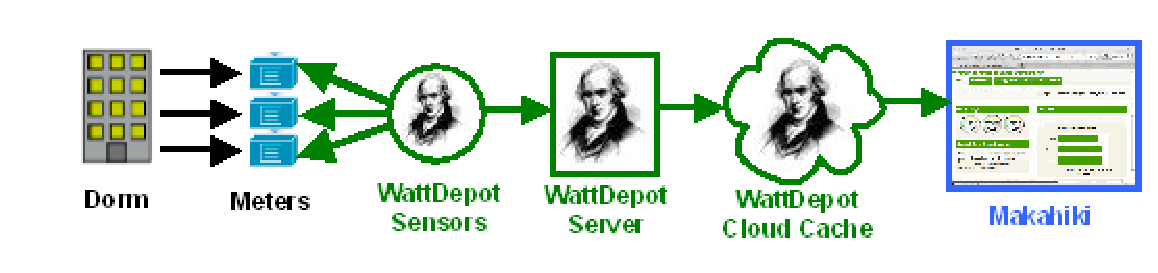
\includegraphics[width=0.8\textwidth]{architecture.eps}
  \caption{\em \small System Architecture: Dorm energy usage is captured by one or more meters, which 
are queried by WattDepot sensors and the raw data sent to the WattDepot server. Analyses are computed
and stored in cloud-based services for ease of retrieval and display in the Makahiki web application.}
  \label{fig:architecture}
\end{figure*} 

Figure \ref{fig:architecture} illustrates the high-level architecture of
the system. There are three basic subsystems in this architecture.  The
first is the dorm electrical infrastructure, illustrated on the left hand
side of the diagram.  This infrastructure includes power distribution to
dorm rooms where residents consume power.  It also includes one or more
electrical meters that monitor power consumption and that are connected to
the Internet.  The second subsystem is WattDepot, an open source suite of
tools we have developed for enterprise-level collection, storage, analysis,
and presentation of energy data. The third subsystem is Makahiki, an open
source framework for building dorm energy competition web applications.
The following sections discuss each of these architectural components in
more detail.

\subsubsection{WattDepot Sensors}

Electricity can be generated and/or consumed by a wide variety of devices
and monitored by a wide variety of metering technologies.  Many energy
management software systems are tied to a particular energy device and/or
meter; indeed, they are often marketed as an accessory to the hardware.
For example, most commercial energy meter manufacturers provide software
for storing data about the power generated by the meter and simple
visualizations of the power generated over time.

Our architecture attempts to make the software as independent from
the energy hardware devices as possible.  To achieve this independence, the
WattDepot architecture includes ``sensors'', or small software processes
that query any given energy device according to its native protocol,
collect standard information, and then send it to a WattDepot server using
the Internet and the RESTful WattDepot API over HTTP.  This design means
that new energy devices can be integrated easily into the WattDepot
software ecosystem just by writing the sensor interface.  The use of a
RESTful HTTP protocol for communication with the WattDepot server means
that the sensor can be implemented in any programming language.

We have implemented WattDepot sensors for the TED 5000 home energy device, 
the Veris power meter collected through the Building Manager Online system,
and for the Acuvim and Shark commercial energy meters. The latter sensors
are based upon the standard ModBus/TCP protocol. 

Sensors transmit data to a WattDepot server using a standardized, published
protocol, as discussed next.

\subsubsection{WattDepot Server}

A WattDepot server accepts raw energy data from devices (via sensors) and
makes this data (or analyses based upon it) available to clients.  The
WattDepot server implements a variety of design decisions intended to
improve its generality, reusability, and extensibility, including: (1) a
RESTful API, (2) a pluggable back-end database, (3) aggregation via
``virtual'' sources, (4) data interpolation, and (5) multiple
representations.

{\em RESTful API.} WattDepot conforms to modern web service design best
practices by providing a RESTful API.  REST (REpresentational State
Transfer) \cite{REST} is a specification paradigm, which, when applied to
web services, generally results in more easily usable and extensible
communication than alternatives such as SOAP. The details of RESTful design
are beyond the scope of this paper. Some of the implications include
URLs that can serve as unique identifiers for energy data and the use of HTTP
methods such as PUT, POST, GET, and DELETE to add, amend, retrieve, and
delete energy data. The WattDepot API \cite{WattDepotAPI} provides more
details and a full specification of the supported operations.

{\em Pluggable back-end database.} The WattDepot server implements an
abstraction layer that enables the server to be built with a variety of
different persistence mechanisms.  By default, WattDepot uses the Apache
Derby relational database, which is a high performance, embedded database
written in Java.  However, WattDepot can be ported to other relational or
non-relational database systems by implementing an interface and setting some 
run-time configuration parameters. 

{\em Aggregation via virtual sources.} The data from a single physical
meter is generally represented in WattDepot as a ``Source''.  Each
WattDepot Source can indicate the power generated or consumed by that
device at any moment in time, the energy generated or consumed by that
device over a period of time, the carbon intensity associated with that
device, and other features.  In addition to this one-to-one correspondence,
WattDepot also supports the definition of ``virtual'' Sources, which are
Sources defined as the aggregation of other Sources.  For example, a floor
on a building might have two meters collecting energy consumption data for
the two sections of the floor.  WattDepot allows users to
define a virtual Source representing the aggregation of the data stream
from the two meters.  This virtual Source thus represents the total energy
consumption for the floor. Virtual Sources can be arranged in a hierarchy,
such that the virtual Sources for each floor in the building can themselves
be contained in a virtual Source representing the entire building's energy
consumption.

{\em Data interpolation.} One common initial roadblock to analyzing energy
data collected from multiple sources is the ``timestamp problem''. For
example, assume that energy consumption on a building floor is collected by
two meters, and that energy data is collected from those meters becomes
available approximately every 15 minutes, but the timestamps associated
with the data for a given time period differ by a minute or two.
Determining the aggregate energy consumption is no longer a simple matter
of importing the two data sets into a spreadsheet and using a summation
macro, because the timestamps from the two meters do not ``match up''.
WattDepot addresses this problem by providing automatic interpolation. For
example, assume a meter sent energy data at roughly 30 minute intervals:
11:23 AM, 11:56 AM, 12:25 PM, and 1:01 PM.  You can request the energy consumed
by this Source between 12:00 PM and 1:00 PM, for example, and WattDepot will
automatically interpolate the raw data values to provide an estimate for
the interval of interest.  Automatic linear interpolation enables virtual Sources
to return reasonable values even when its constituent Sources send data at
different times and with different frequencies. 

{\em Multiple representations.} One benefit of a RESTful architecture is
the separation of a ``resource'' from its ``representation''.  In
WattDepot, this separation means that data and analyses for a given Source can
be provided in different ways, depending upon the needs of the client.  So
far, WattDepot can provide data to clients using XML, JSON (the format
supported by Google Visualizations), and CSV (comma-separated values),
which is useful for importing WattDepot data into other tools for
additional analysis.

\subsubsection{WattDepot Cloud Cache}

A typical dorm energy competition will involve hundreds to thousands of
students.  Energy data requests are characterized by the desire for
relatively recent results. For example, how much power did my dorm use in
the last hour, and how does that compare to usage during the same hour over
the past month? They are also characterized by the fact that those same
results do not tend to be user-specific: monitoring the energy usage of
individual dorm members is not practical at the current time; the most
fine-grained collection we have seen is floor-level. These two application
characteristics argue for caching of results so that the WattDepot server
is not processing the same request hundreds or thousands of times.

The architectural issue is: where should that cache of reusable data be
placed?  There are three choices: in the server, in the web application, or
in a third service ``in between'' the server and the web application.
All of these approaches have their strengths and weaknesses.  Our system
architecture chooses the last approach, in which a service called
WattDepot-GData creates Google Docs spreadsheets containing high level
abstractions of the raw data stored in the WattDepot server.  We chose the
Google Docs cloud-based storage system because it is free, it is scalable
and very high performance, and it integrates extremely well with the Google
Visualization API.  This latter feature enables the Makahiki web
application framework to provide advanced, interactive visualizations of
energy data with very little end-user coding.

\subsubsection{Makahiki}

\begin{figure*}[!th]
  \center
  \includegraphics[width=0.8\textwidth]{makahiki.eps}
  \caption{\em \small An example dorm energy web application built with Makahiki.}
  \label{fig:makahiki}
\end{figure*} 

The final subsystem in our architecture is called Makahiki \cite{makahiki-site}, which is a
framework for developing dorm energy competition web applications.  Figure
\ref{fig:makahiki} illustrates the home page for the University of Hawaii
dorm energy web application built as a configuration of Makahiki. As a
framework, Makahiki supports several forms of tailoring without requiring
any editing of the underlying Python source code.

{\em Configurable look and feel.} The color scheme and logos for the site
are defined in CSS files that can be edited or replaced to best reflect the
University's color scheme. At the University of Hawaii, Makahiki is
configured with a green and white color scheme and the ``Kukui Cup'' name
and logo.   We use the JQuery ThemeRoller application to simplify the generation of 
alternative look and feels.

{\em Configurable display panes.} Each page in the web application generated by Makahiki
contains a number of display panes. The contents of these display panes can be easily 
reconfigured. For example, the form of energy visualization can be changed by editing 
the underlying Javascript associated with the display pane. 

{\em Configurable functional modes.}  Makahiki supports several functional ``modes'', which 
enable it to conform to the needs of a wide variety of dorm energy competitions.  

The ``single page'' mode is the simplest mode, which enables a university
to create a simple, single page website with a matching look and feel for
their university.  In single page mode, energy data and dorm standings can
be visualized by manually creating Google Docs spreadsheets and configuring
the display panes to visualize the data as tables or bar charts.  In this
basic functional mode, there need not be any use of WattDepot; all data can
be collected manually by competition organizers and entered into
spreadsheets for display.

In ``multi page'' mode, Makahiki generates a web application containing a
Home page, a Resources page, an Energy data page, a Competition page, and
an About page.  Multi page mode provides a more comprehensive web
application that enables the university to provide significantly more
information than is possible with single page mode.  As with single page
mode, multi page mode does not require WattDepot.

The final mode is called ``login'' mode, and it is in this mode that
Makahiki provides features not currently found in other dorm energy
competition web applications.  In this mode, each resident of the dorm can
login to their own personally customized home page, which provides access
to energy data regarding their floor as well as behavioral change tools.
Login mode requires automated access to energy data and so WattDepot is
required.  Figure \ref{fig:makahiki-login} illustrates a sample
configuration of an individual user home page.

\begin{figure*}[!th]
  \center
  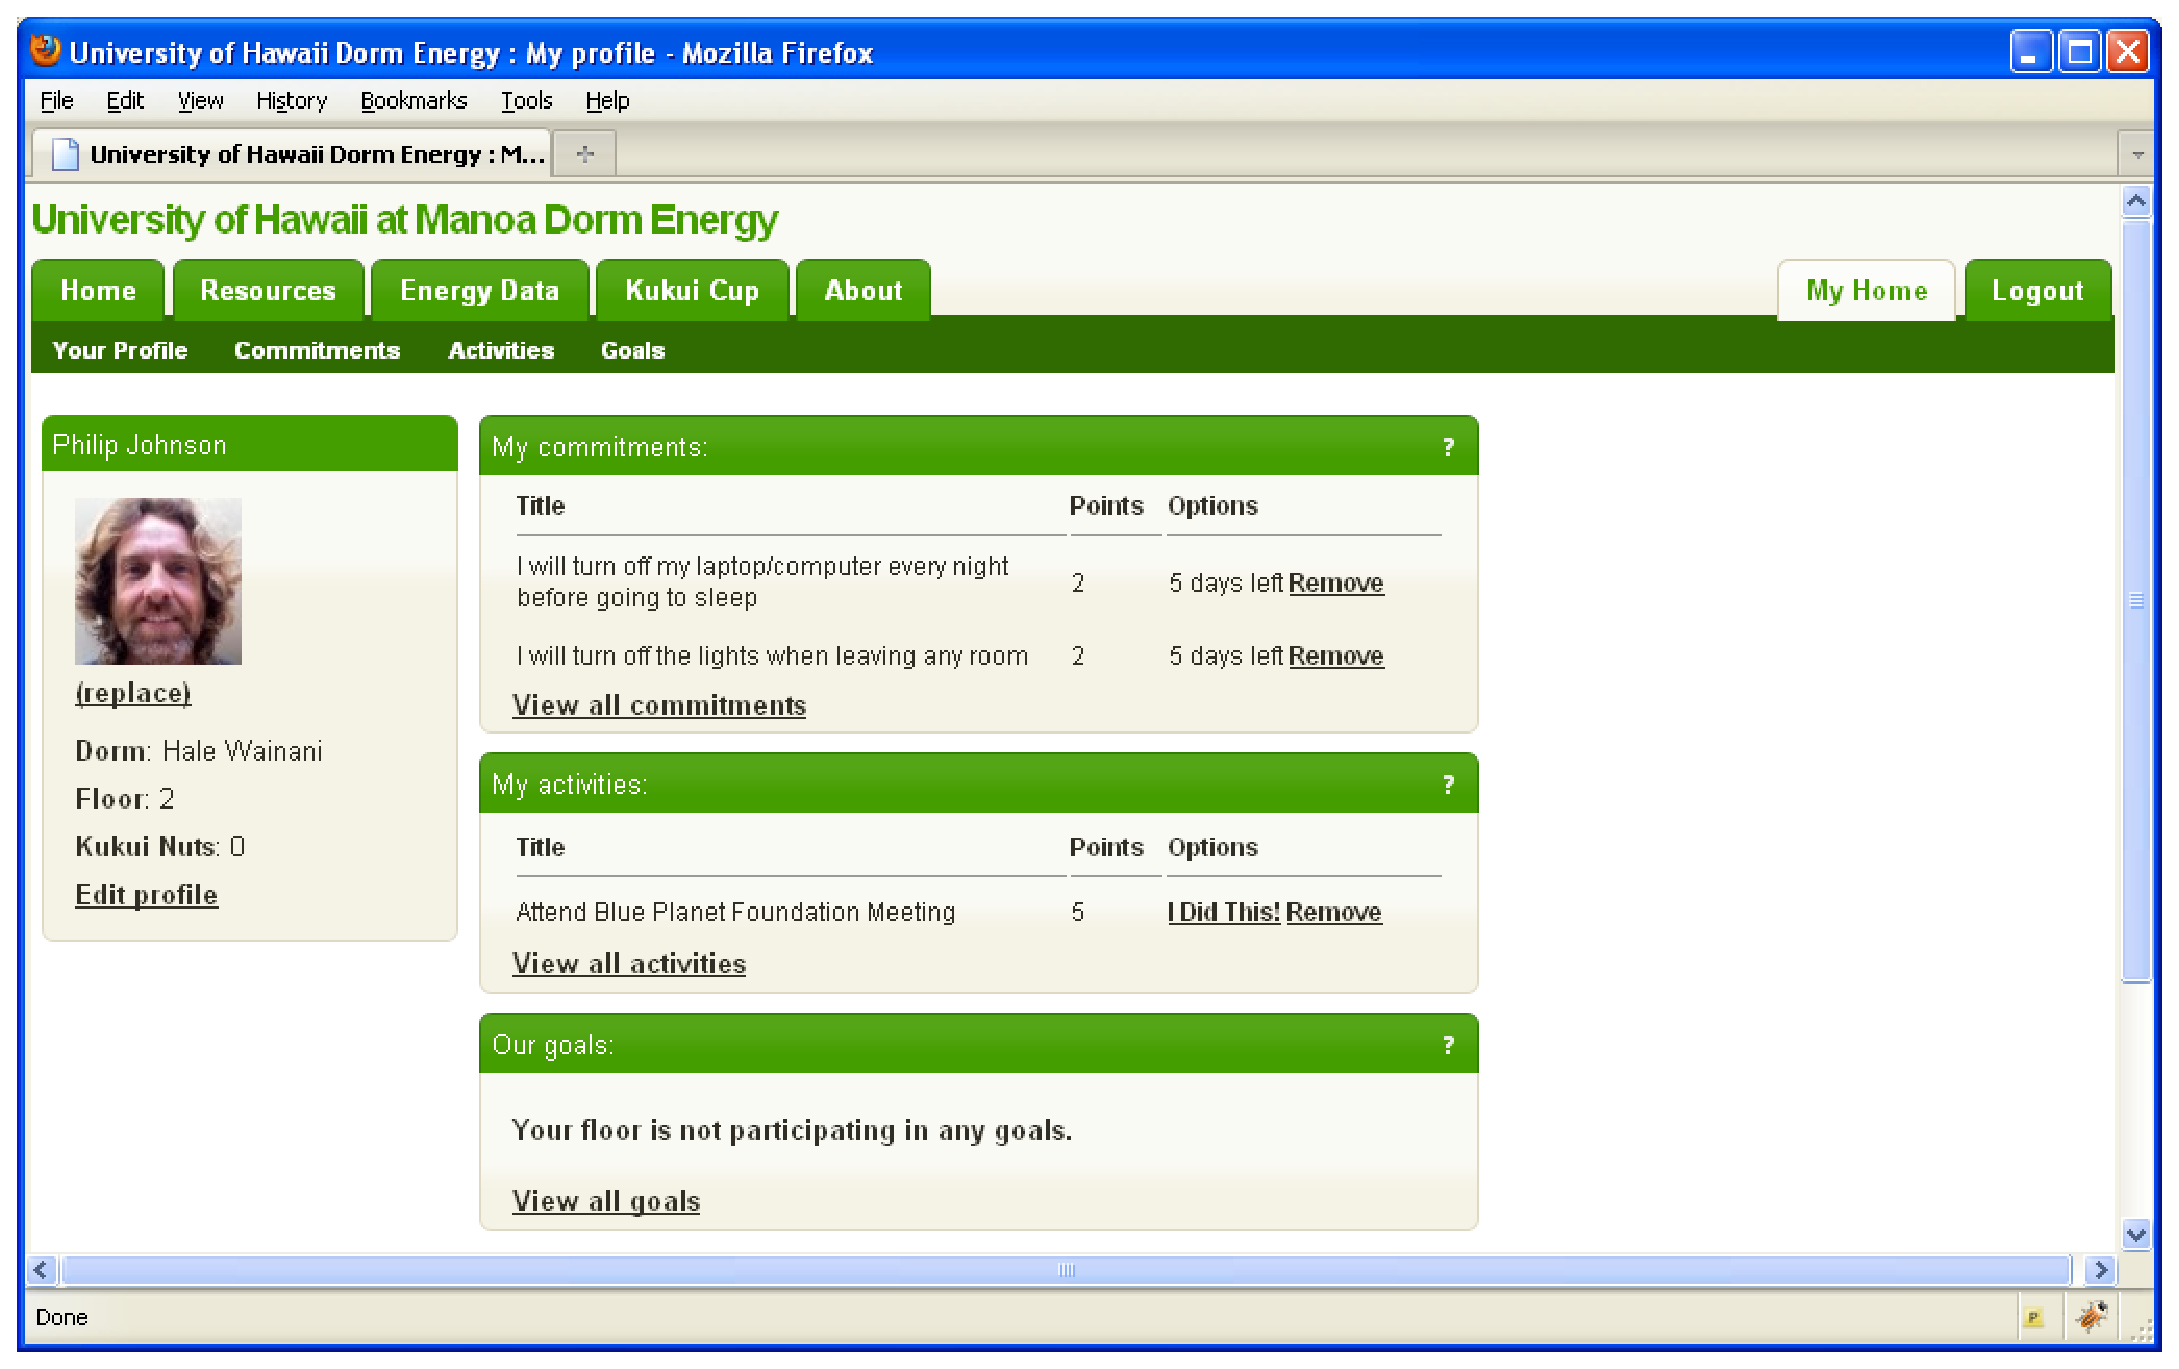
\includegraphics[width=0.8\textwidth]{makahiki.login.eps}
  \caption{\em \small The personalized user home page with floor-level monitoring and behavioral change tools 
including commitments, activities, and goals.}
  \label{fig:makahiki-login}
\end{figure*} 

The design of Makahiki's login mode is based upon research findings
regarding behavioral change in energy consumption, which indicate that
feedback, commitments, goal setting, knowledge, and incentives are all
important mechanisms to create sustained change.  Makahiki provides
feedback regarding energy usage via near-real time data on the user's
floor's cumulative energy usage during the competition, instantaneous power
consumption, and comparisons to baseline measures and other
floors. Activities are individual, concrete actions such as attending a
meeting or movie showing about energy, watching an energy-related video, or
reading news articles, all of which are designed to heighten the student's
knowledge and awareness of energy. Commitments are more general changes in
behavior, such as turning off the lights when leaving any room.  Finally,
goals are behaviors involving the floor as a whole, such as attempting to
reduce energy usage by 10\% over the next week.  

To incentivize participation in activities, goals, and commitments,
Makahiki provides the capability for users to accumulate points for
completing instances of these three types of actions.  Makahiki supports
verification of activities and goals. When defining an activity for
inclusion in the system (such as the watching of a short YouTube video on
wind energy), the site administrator also can enter several short questions
whose answers are found in the video (such as ``What is the average power
output of the wind turbine in the video?'').  When a user requests to
receive points for having performed that activity, the system will prompt
the user with a question selected at random.  The user's request, with
their answer, is reviewed by administrators who can decide whether or not
to confirm or deny the request.  

Commitments, while an important tool for behavioral change, are problematic
to verify.  Makahiki addresses this issue in several ways.  First,
commitments are worth less points than verifiable activities or goals.
Second, commitments are active for a period of five days, and when the user
requests points at the end of that time, they must self-verify that they
satisfied the commitment.  Finally, and most importantly, commitments are
public: the Makahiki website (and associated technologies such as an
electronic billboard in the lobby of the dorms and Facebook page
integration) broadcasts the commitments entered into by the users. Research
shows that making public commitments are a powerful incentive for
behavioral change.





















%%%%%%%%%%%%%%%%%%%%%%%%%%%%%% -*- Mode: Latex -*- %%%%%%%%%%%%%%%%%%%%%%%%%%%%
%% 10-07-experiment.tex --  HICSS 44 Kukui Cup paper
%% Author          : Philip Johnson
%% Created On      : Mon Sep 23 11:52:28 2002
%% Last Modified By: Philip Johnson
%% Last Modified On: Thu Jun 10 15:05:36 2010
%%%%%%%%%%%%%%%%%%%%%%%%%%%%%%%%%%%%%%%%%%%%%%%%%%%%%%%%%%%%%%%%%%%%%%%%%%%%%%%
%%   Copyright (C) 2009 Philip Johnson
%%%%%%%%%%%%%%%%%%%%%%%%%%%%%%%%%%%%%%%%%%%%%%%%%%%%%%%%%%%%%%%%%%%%%%%%%%%%%%%
%% 

\section{Evaluation}
\label{sec:evaluation}

Our work addresses the following research questions:

\begin{enumerate}
	\item To what extent and in what ways does our dorm energy competition impact the ``energy literacy'' of participating students?
	\item How effective is our use of information technology to support behavioral change tools?
	\item To what extent does our approach yield sustained changes in energy behavior, and what factors appear to influence sustained change?
\end{enumerate}

To find the answers to these questions, we have planned a dorm energy competition for Fall 2010 semester at the University of Hawai`i at M\=anoa. The rest of this section describes the competition design, the data we plan to gather, and how we intend to analyze the data.

\subsection{Competition design}

The competition is planned to take place in multiple freshman dormitories on the M\=anoa campus. Freshmen have been targeted since they are deemed more likely to participate in dormitory events, they are a ``renewable resource'', and past research has shown that freshmen perform well in these competitions \cite{petersen-dorm-energy-reduction}. There are 10 floors per residence hall, with 26 residents per floor at full occupancy, resulting in 260 potential participants per building.

The competition will take place over three weeks in the Fall 2010 semester. Each of the first two weeks will constitute a separate round of the competition, while the results from the final week apply only to the overall competition. Structuring the competition into rounds ensures that residents that did not participate initially can start participating in a later round without undue disadvantage.

The energy usage of the participants will be measured using power meters we will install in the central electrical panels on the floors of the dorms. Due to the architectural design and electrical infrastructure of the buildings, the meters will measure the energy consumption of each pair of floors. The meters to be installed will support sampling every 15 seconds, enabling near-realtime energy feedback display. The meter data will be stored using WattDepot.

There will be two scores for the competition: energy consumption and Kukui Nut points. Energy consumption is the total amount of electrical energy consumed by a pair of floors in kWh during a round as measured by the power meters, so lower energy consumption scores are better. Kukui Nut points are awarded through the competition website (powered by Makahiki) for the completion of tasks intended to increase participants' energy literacy or reduce energy usage. Kukui Nut points are awarded to individuals through the website (though they can also be aggregated at the floor or dorm level), but the energy consumption is only recorded at the floor level. We will provide awards based on energy consumption (at floor and dormitory levels), and Kukui Nut points (at individual, floor, and dormitory levels), many with associated prizes to incentivize participation.

In addition to the information technology support of the competition, we will deploy a variety of other methods to engage residents in the competition, such as a kick-off meeting for each dorm where free T-shirts will be distributed, buttons to be distributed to all residents, signage on each floor about the competition, and closing grand prize ceremony.

\subsection{Data sources}

We plan to collect a variety of types of data from the competition. We will record both instantaneous power and cumulative energy consumed on a floor by floor basis for each residence hall, both before the competition starts and continuing for at least 6 months after the competition ends. The sampling rate will be a minimum of 1 minute outside the competition period, and a maximum of 1 minute during the competition period (with a target of 15 seconds), with both rates kept constant during the study to the degree possible.

The energy literacy of participants will be assessed at the start and end of the competition. The assessment will be through a questionnaire that is presented to participants via the contest website as an activity that can be performed for Kukui Nut points. The pre-competition questionnaire will be made available only in the first week of the competition, while the post-competition questionnaire will be made available only in the final week of the competition. Since the website-administered questionnaire is simply a task that can selected by participants, there is the potential that only those participants that feel that they are energy literate will participate in the survey, leading to bias. For this reason, in addition to administration through the website, the questionnaire will be administered in person on paper to two randomly-selected floors.

The competition website will log data about participants' actions on the site. All participant actions and events will be logged with a timestamp. Some example events are: logging into website, selecting a goal for floor participation, and submitting text to verify completion of an activity. These events can be used to create a profile of each participant.

After the competition has ended, participants that used the website will be emailed a link to a qualitative questionnaire. This questionnaire will ask for participants' assessment of the competition, the website, and energy literacy in general.

In early in the following semester (February 2011), the power data for floors will be re-examined to see whether conservation begun as part of the competition has been sustained months later. Floors with particularly high sustained conservation (compared to pre-competition average floor power), and those with low or non-conservation will be selected for an additional questionnaire, and possible face-to-face interviews to determine residents' self-assessment about why they were or were not sustaining the conservation gains made during the competition.

\subsection{Analysis}

Using the energy literacy surveys from before and after the competition, we can 
address the first research question: the impact of the competition on the energy literacy of the participants. Increased scores in post-competition energy literacy would provide an indication that the activities of the competition may increase energy literacy. We will also examine the opposite relationship, to see how the energy literacy of a pair of floors correlates to the energy consumption of those floors during the competition.

There are several ways to address the second research question: the effectiveness of our information technology to support behavioral change tools. One basic metric will be to examine the website logs to see how many residents actually participate in the competition by logging into the website, how often they log in, and how many tasks they complete. The effectiveness of the tasks in improving energy literacy will be assessed by examining the correlation between Kukui Nut points awarded per participant, and their performance on the energy literacy surveys. The relationship between a floor's energy usage and its aggregated Kukui Nut points will provide another window into the effectiveness of the information technology to support behavior change.

The third research question is to what extent does our approach yield sustained changes in energy behavior, and what factors appear to influence sustained change? Using the energy data, we can determine the energy consumption of each pair of floors before, during, and after the competition. The energy consumption after the competition ends is most important when looking for sustained change, and we will look at the relationship between energy consumption and Kukui Nut points, website use, and energy literacy.
%%%%%%%%%%%%%%%%%%%%%%%%%%%%%% -*- Mode: Latex -*- %%%%%%%%%%%%%%%%%%%%%%%%%%%%
%% 10-07-future.tex --  HICSS 44 Kukui Cup paper
%% Author          : Philip Johnson
%% Created On      : Mon Sep 23 11:52:28 2002
%% Last Modified By: Philip Johnson
%% Last Modified On: Mon Jun 14 12:55:47 2010
%%%%%%%%%%%%%%%%%%%%%%%%%%%%%%%%%%%%%%%%%%%%%%%%%%%%%%%%%%%%%%%%%%%%%%%%%%%%%%%
%%   Copyright (C) 2009 Philip Johnson
%%%%%%%%%%%%%%%%%%%%%%%%%%%%%%%%%%%%%%%%%%%%%%%%%%%%%%%%%%%%%%%%%%%%%%%%%%%%%%%
%% 

\section{Future Directions}
\label{sec:future-directions}

As noted above, we are currently planning for the inaugural Kukui Cup
competition to take place in October, 2010.  In addition, we are planning
several other extensions to this research.

First, we are interested in adapting this technology and research approach
to the issue of residential energy consumption.  Residential energy
consumption differs in many ways from dorm energy consumption. Most
significantly, residential energy users are billed directly for the energy
use, so there is an important financial incentive for conservation.
However, the research indicates that tools such as goals and public
commitments remain important in the residential energy application domain.

Second, we would like to support the use of Makahiki as a framework for
other universities who desire to implement a dorm energy competition.  We
believe that Makahiki can significantly lower the ``barrier to entry'' for
universities, and allows them to get started with a simple site if required. 

Third, we are excited by the possibility of integrating grid-level
information into WattDepot for use by Makahiki and other high level
applications.  For example, we are working with our local utility to
provide WattDepot with information on the current mix of generation sources
(i.e. coal, oil, nuclear, solar, wind, etc.) and their aggregate output
(i.e. grid load).  Given this information, it would be possible for
WattDepot to provide the carbon intensity associated with the energy
consumed by end-users at any point in time.  This would make it possible
for the Kukui Cup to incentivize behaviors such as ``doing laundry when the
carbon intensity of the grid is low.''







\section{Acknowledgments}

Financial support for this research is provided by the Renewable Energy and
Island Sustainability (REIS) project at the University of Hawai`i at M\=anoa.

\bibliographystyle{IEEEtran}
\bibliography{smartconsumer,sustainability}
\end{document}






